\documentclass[twoside]{book}

% Packages required by doxygen
\usepackage{fixltx2e}
\usepackage{calc}
\usepackage{doxygen}
\usepackage[export]{adjustbox} % also loads graphicx
\usepackage{graphicx}
\usepackage[utf8]{inputenc}
\usepackage{makeidx}
\usepackage{multicol}
\usepackage{multirow}
\PassOptionsToPackage{warn}{textcomp}
\usepackage{textcomp}
\usepackage[nointegrals]{wasysym}
\usepackage[table]{xcolor}

% Font selection
\usepackage[T1]{fontenc}
\usepackage[scaled=.90]{helvet}
\usepackage{courier}
\usepackage{amssymb}
\usepackage{sectsty}
\renewcommand{\familydefault}{\sfdefault}
\allsectionsfont{%
  \fontseries{bc}\selectfont%
  \color{darkgray}%
}
\renewcommand{\DoxyLabelFont}{%
  \fontseries{bc}\selectfont%
  \color{darkgray}%
}
\newcommand{\+}{\discretionary{\mbox{\scriptsize$\hookleftarrow$}}{}{}}

% Page & text layout
\usepackage{geometry}
\geometry{%
  a4paper,%
  top=2.5cm,%
  bottom=2.5cm,%
  left=2.5cm,%
  right=2.5cm%
}
\tolerance=750
\hfuzz=15pt
\hbadness=750
\setlength{\emergencystretch}{15pt}
\setlength{\parindent}{0cm}
\setlength{\parskip}{3ex plus 2ex minus 2ex}
\makeatletter
\renewcommand{\paragraph}{%
  \@startsection{paragraph}{4}{0ex}{-1.0ex}{1.0ex}{%
    \normalfont\normalsize\bfseries\SS@parafont%
  }%
}
\renewcommand{\subparagraph}{%
  \@startsection{subparagraph}{5}{0ex}{-1.0ex}{1.0ex}{%
    \normalfont\normalsize\bfseries\SS@subparafont%
  }%
}
\makeatother

% Headers & footers
\usepackage{fancyhdr}
\pagestyle{fancyplain}
\fancyhead[LE]{\fancyplain{}{\bfseries\thepage}}
\fancyhead[CE]{\fancyplain{}{}}
\fancyhead[RE]{\fancyplain{}{\bfseries\leftmark}}
\fancyhead[LO]{\fancyplain{}{\bfseries\rightmark}}
\fancyhead[CO]{\fancyplain{}{}}
\fancyhead[RO]{\fancyplain{}{\bfseries\thepage}}
\fancyfoot[LE]{\fancyplain{}{}}
\fancyfoot[CE]{\fancyplain{}{}}
\fancyfoot[RE]{\fancyplain{}{\bfseries\scriptsize Generated by Doxygen }}
\fancyfoot[LO]{\fancyplain{}{\bfseries\scriptsize Generated by Doxygen }}
\fancyfoot[CO]{\fancyplain{}{}}
\fancyfoot[RO]{\fancyplain{}{}}
\renewcommand{\footrulewidth}{0.4pt}
\renewcommand{\chaptermark}[1]{%
  \markboth{#1}{}%
}
\renewcommand{\sectionmark}[1]{%
  \markright{\thesection\ #1}%
}

% Indices & bibliography
\usepackage{natbib}
\usepackage[titles]{tocloft}
\setcounter{tocdepth}{3}
\setcounter{secnumdepth}{5}
\makeindex

% Hyperlinks (required, but should be loaded last)
\usepackage{ifpdf}
\ifpdf
  \usepackage[pdftex,pagebackref=true]{hyperref}
\else
  \usepackage[ps2pdf,pagebackref=true]{hyperref}
\fi
\hypersetup{%
  colorlinks=true,%
  linkcolor=blue,%
  citecolor=blue,%
  unicode%
}

% Custom commands
\newcommand{\clearemptydoublepage}{%
  \newpage{\pagestyle{empty}\cleardoublepage}%
}

\usepackage{caption}
\captionsetup{labelsep=space,justification=centering,font={bf},singlelinecheck=off,skip=4pt,position=top}

%===== C O N T E N T S =====

\begin{document}

% Titlepage & ToC
\hypersetup{pageanchor=false,
             bookmarksnumbered=true,
             pdfencoding=unicode
            }
\pagenumbering{roman}
\begin{titlepage}
\vspace*{7cm}
\begin{center}%
{\Large My Project }\\
\vspace*{1cm}
{\large Generated by Doxygen 1.8.11}\\
\end{center}
\end{titlepage}
\clearemptydoublepage
\tableofcontents
\clearemptydoublepage
\pagenumbering{arabic}
\hypersetup{pageanchor=true}

%--- Begin generated contents ---
\chapter{Hierarchical Index}
\section{Class Hierarchy}
This inheritance list is sorted roughly, but not completely, alphabetically\+:\begin{DoxyCompactList}
\item Callback\begin{DoxyCompactList}
\item \contentsline{section}{com.\+initi.\+thierry.\+colormatchapp\+\_\+v02.\+Game\+Surface}{\pageref{classcom_1_1initi_1_1thierry_1_1colormatchapp__v02_1_1_game_surface}}{}
\end{DoxyCompactList}
\item \contentsline{section}{com.\+initi.\+thierry.\+colormatchapp\+\_\+v02.\+High\+Score\+Data}{\pageref{classcom_1_1initi_1_1thierry_1_1colormatchapp__v02_1_1_high_score_data}}{}
\item On\+Click\+Listener\begin{DoxyCompactList}
\item \contentsline{section}{com.\+initi.\+thierry.\+colormatchapp\+\_\+v02.\+Game\+Result\+Activity}{\pageref{classcom_1_1initi_1_1thierry_1_1colormatchapp__v02_1_1_game_result_activity}}{}
\item \contentsline{section}{com.\+initi.\+thierry.\+colormatchapp\+\_\+v02.\+Main\+Activity}{\pageref{classcom_1_1initi_1_1thierry_1_1colormatchapp__v02_1_1_main_activity}}{}
\end{DoxyCompactList}
\item On\+Touch\+Listener\begin{DoxyCompactList}
\item \contentsline{section}{com.\+initi.\+thierry.\+colormatchapp\+\_\+v02.\+Game\+Activity}{\pageref{classcom_1_1initi_1_1thierry_1_1colormatchapp__v02_1_1_game_activity}}{}
\item \contentsline{section}{com.\+initi.\+thierry.\+colormatchapp\+\_\+v02.\+Game\+Surface}{\pageref{classcom_1_1initi_1_1thierry_1_1colormatchapp__v02_1_1_game_surface}}{}
\end{DoxyCompactList}
\item \contentsline{section}{com.\+initi.\+thierry.\+colormatchapp\+\_\+v02.\+Point}{\pageref{classcom_1_1initi_1_1thierry_1_1colormatchapp__v02_1_1_point}}{}
\item Runnable\begin{DoxyCompactList}
\item \contentsline{section}{com.\+initi.\+thierry.\+colormatchapp\+\_\+v02.\+Game\+Surface}{\pageref{classcom_1_1initi_1_1thierry_1_1colormatchapp__v02_1_1_game_surface}}{}
\end{DoxyCompactList}
\item Activity\begin{DoxyCompactList}
\item \contentsline{section}{com.\+initi.\+thierry.\+colormatchapp\+\_\+v02.\+Game\+Activity}{\pageref{classcom_1_1initi_1_1thierry_1_1colormatchapp__v02_1_1_game_activity}}{}
\item \contentsline{section}{com.\+initi.\+thierry.\+colormatchapp\+\_\+v02.\+Game\+Result\+Activity}{\pageref{classcom_1_1initi_1_1thierry_1_1colormatchapp__v02_1_1_game_result_activity}}{}
\item \contentsline{section}{com.\+initi.\+thierry.\+colormatchapp\+\_\+v02.\+Main\+Activity}{\pageref{classcom_1_1initi_1_1thierry_1_1colormatchapp__v02_1_1_main_activity}}{}
\end{DoxyCompactList}
\item Broadcast\+Receiver\begin{DoxyCompactList}
\item \contentsline{section}{com.\+initi.\+thierry.\+colormatchapp\+\_\+v02.\+Game\+Activity.\+Message\+Handler}{\pageref{classcom_1_1initi_1_1thierry_1_1colormatchapp__v02_1_1_game_activity_1_1_message_handler}}{}
\end{DoxyCompactList}
\item S\+Q\+Lite\+Open\+Helper\begin{DoxyCompactList}
\item \contentsline{section}{com.\+initi.\+thierry.\+colormatchapp\+\_\+v02.\+Database\+Operations}{\pageref{classcom_1_1initi_1_1thierry_1_1colormatchapp__v02_1_1_database_operations}}{}
\end{DoxyCompactList}
\item Surface\+View\begin{DoxyCompactList}
\item \contentsline{section}{com.\+initi.\+thierry.\+colormatchapp\+\_\+v02.\+Game\+Surface}{\pageref{classcom_1_1initi_1_1thierry_1_1colormatchapp__v02_1_1_game_surface}}{}
\end{DoxyCompactList}
\end{DoxyCompactList}

\chapter{Class Index}
\section{Class List}
Here are the classes, structs, unions and interfaces with brief descriptions\+:\begin{DoxyCompactList}
\item\contentsline{section}{\hyperlink{classcom_1_1initi_1_1thierry_1_1colormatchapp__v02_1_1_database_operations}{com.\+initi.\+thierry.\+colormatchapp\+\_\+v02.\+Database\+Operations} }{\pageref{classcom_1_1initi_1_1thierry_1_1colormatchapp__v02_1_1_database_operations}}{}
\item\contentsline{section}{\hyperlink{classcom_1_1initi_1_1thierry_1_1colormatchapp__v02_1_1_game_activity}{com.\+initi.\+thierry.\+colormatchapp\+\_\+v02.\+Game\+Activity} }{\pageref{classcom_1_1initi_1_1thierry_1_1colormatchapp__v02_1_1_game_activity}}{}
\item\contentsline{section}{\hyperlink{classcom_1_1initi_1_1thierry_1_1colormatchapp__v02_1_1_game_result_activity}{com.\+initi.\+thierry.\+colormatchapp\+\_\+v02.\+Game\+Result\+Activity} }{\pageref{classcom_1_1initi_1_1thierry_1_1colormatchapp__v02_1_1_game_result_activity}}{}
\item\contentsline{section}{\hyperlink{classcom_1_1initi_1_1thierry_1_1colormatchapp__v02_1_1_game_surface}{com.\+initi.\+thierry.\+colormatchapp\+\_\+v02.\+Game\+Surface} }{\pageref{classcom_1_1initi_1_1thierry_1_1colormatchapp__v02_1_1_game_surface}}{}
\item\contentsline{section}{\hyperlink{classcom_1_1initi_1_1thierry_1_1colormatchapp__v02_1_1_high_score_data}{com.\+initi.\+thierry.\+colormatchapp\+\_\+v02.\+High\+Score\+Data} }{\pageref{classcom_1_1initi_1_1thierry_1_1colormatchapp__v02_1_1_high_score_data}}{}
\item\contentsline{section}{\hyperlink{classcom_1_1initi_1_1thierry_1_1colormatchapp__v02_1_1_main_activity}{com.\+initi.\+thierry.\+colormatchapp\+\_\+v02.\+Main\+Activity} }{\pageref{classcom_1_1initi_1_1thierry_1_1colormatchapp__v02_1_1_main_activity}}{}
\item\contentsline{section}{\hyperlink{classcom_1_1initi_1_1thierry_1_1colormatchapp__v02_1_1_game_activity_1_1_message_handler}{com.\+initi.\+thierry.\+colormatchapp\+\_\+v02.\+Game\+Activity.\+Message\+Handler} }{\pageref{classcom_1_1initi_1_1thierry_1_1colormatchapp__v02_1_1_game_activity_1_1_message_handler}}{}
\item\contentsline{section}{\hyperlink{classcom_1_1initi_1_1thierry_1_1colormatchapp__v02_1_1_point}{com.\+initi.\+thierry.\+colormatchapp\+\_\+v02.\+Point} }{\pageref{classcom_1_1initi_1_1thierry_1_1colormatchapp__v02_1_1_point}}{}
\end{DoxyCompactList}

\chapter{Class Documentation}
\hypertarget{classcom_1_1initi_1_1thierry_1_1colormatchapp__v02_1_1_database_operations}{}\section{com.\+initi.\+thierry.\+colormatchapp\+\_\+v02.\+Database\+Operations Class Reference}
\label{classcom_1_1initi_1_1thierry_1_1colormatchapp__v02_1_1_database_operations}\index{com.\+initi.\+thierry.\+colormatchapp\+\_\+v02.\+Database\+Operations@{com.\+initi.\+thierry.\+colormatchapp\+\_\+v02.\+Database\+Operations}}
Inheritance diagram for com.\+initi.\+thierry.\+colormatchapp\+\_\+v02.\+Database\+Operations\+:\begin{figure}[H]
\begin{center}
\leavevmode
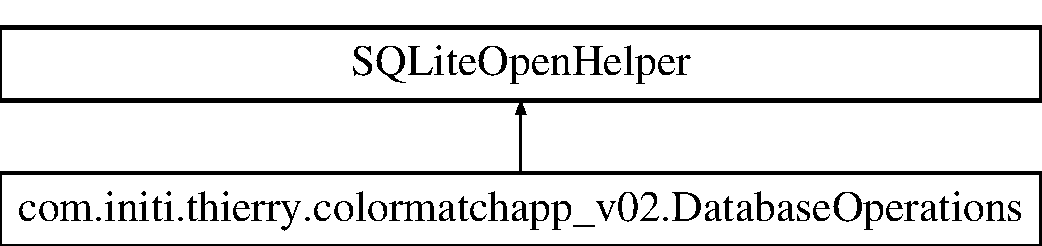
\includegraphics[height=2.000000cm]{classcom_1_1initi_1_1thierry_1_1colormatchapp__v02_1_1_database_operations}
\end{center}
\end{figure}
\subsection*{Public Member Functions}
\begin{DoxyCompactItemize}
\item 
{\bfseries Database\+Operations} (Context context)\hypertarget{classcom_1_1initi_1_1thierry_1_1colormatchapp__v02_1_1_database_operations_a8c4fe0ff81536dd697c1fd6c959155e3}{}\label{classcom_1_1initi_1_1thierry_1_1colormatchapp__v02_1_1_database_operations_a8c4fe0ff81536dd697c1fd6c959155e3}

\item 
void {\bfseries on\+Create} (S\+Q\+Lite\+Database db)\hypertarget{classcom_1_1initi_1_1thierry_1_1colormatchapp__v02_1_1_database_operations_a95c099d7c28a99c8c11fd9c2d082c371}{}\label{classcom_1_1initi_1_1thierry_1_1colormatchapp__v02_1_1_database_operations_a95c099d7c28a99c8c11fd9c2d082c371}

\item 
void {\bfseries on\+Upgrade} (S\+Q\+Lite\+Database db, int old\+Version, int new\+Version)\hypertarget{classcom_1_1initi_1_1thierry_1_1colormatchapp__v02_1_1_database_operations_a357371e4b1022b4a6d836409740a8d44}{}\label{classcom_1_1initi_1_1thierry_1_1colormatchapp__v02_1_1_database_operations_a357371e4b1022b4a6d836409740a8d44}

\item 
void {\bfseries insert\+Information} (\hyperlink{classcom_1_1initi_1_1thierry_1_1colormatchapp__v02_1_1_database_operations}{Database\+Operations} dop, String name, String date, int score)\hypertarget{classcom_1_1initi_1_1thierry_1_1colormatchapp__v02_1_1_database_operations_a75a93524f17e97642023dcc5cf248edb}{}\label{classcom_1_1initi_1_1thierry_1_1colormatchapp__v02_1_1_database_operations_a75a93524f17e97642023dcc5cf248edb}

\item 
Cursor {\bfseries select\+Information} (\hyperlink{classcom_1_1initi_1_1thierry_1_1colormatchapp__v02_1_1_database_operations}{Database\+Operations} dop)\hypertarget{classcom_1_1initi_1_1thierry_1_1colormatchapp__v02_1_1_database_operations_a30f87ef90139e07d6def8d1fd9919fa1}{}\label{classcom_1_1initi_1_1thierry_1_1colormatchapp__v02_1_1_database_operations_a30f87ef90139e07d6def8d1fd9919fa1}

\end{DoxyCompactItemize}
\subsection*{Public Attributes}
\begin{DoxyCompactItemize}
\item 
String {\bfseries C\+R\+E\+A\+T\+E\+\_\+\+Q\+U\+E\+RY}
\end{DoxyCompactItemize}
\subsection*{Static Public Attributes}
\begin{DoxyCompactItemize}
\item 
static final int {\bfseries database\+Version} = 1\hypertarget{classcom_1_1initi_1_1thierry_1_1colormatchapp__v02_1_1_database_operations_a044c03906d4666706d456c1e40b63507}{}\label{classcom_1_1initi_1_1thierry_1_1colormatchapp__v02_1_1_database_operations_a044c03906d4666706d456c1e40b63507}

\end{DoxyCompactItemize}


\subsection{Detailed Description}
Created by Thierry on 1/1/2016. 

\subsection{Member Data Documentation}
\index{com\+::initi\+::thierry\+::colormatchapp\+\_\+v02\+::\+Database\+Operations@{com\+::initi\+::thierry\+::colormatchapp\+\_\+v02\+::\+Database\+Operations}!C\+R\+E\+A\+T\+E\+\_\+\+Q\+U\+E\+RY@{C\+R\+E\+A\+T\+E\+\_\+\+Q\+U\+E\+RY}}
\index{C\+R\+E\+A\+T\+E\+\_\+\+Q\+U\+E\+RY@{C\+R\+E\+A\+T\+E\+\_\+\+Q\+U\+E\+RY}!com\+::initi\+::thierry\+::colormatchapp\+\_\+v02\+::\+Database\+Operations@{com\+::initi\+::thierry\+::colormatchapp\+\_\+v02\+::\+Database\+Operations}}
\subsubsection[{\texorpdfstring{C\+R\+E\+A\+T\+E\+\_\+\+Q\+U\+E\+RY}{CREATE_QUERY}}]{\setlength{\rightskip}{0pt plus 5cm}String com.\+initi.\+thierry.\+colormatchapp\+\_\+v02.\+Database\+Operations.\+C\+R\+E\+A\+T\+E\+\_\+\+Q\+U\+E\+RY}\hypertarget{classcom_1_1initi_1_1thierry_1_1colormatchapp__v02_1_1_database_operations_af7687136987b9759e38948379d016014}{}\label{classcom_1_1initi_1_1thierry_1_1colormatchapp__v02_1_1_database_operations_af7687136987b9759e38948379d016014}
{\bfseries Initial value\+:}
\begin{DoxyCode}
= \textcolor{stringliteral}{"CREATE TABLE IF NOT EXISTS "}+ HighScoreData.TableInfo.TABLE\_NAME +
            \textcolor{stringliteral}{"("}+ TableInfo.PLAYER\_NAME+\textcolor{stringliteral}{" TEXT, "}+ TableInfo.SCORE\_DATE+\textcolor{stringliteral}{" TEXT , "}+ TableInfo.PLAYER\_SCORE+\textcolor{stringliteral}{"
       INT, "} +
            \textcolor{stringliteral}{"PRIMARY KEY ("}+TableInfo.SCORE\_DATE+\textcolor{stringliteral}{") );"}
\end{DoxyCode}


The documentation for this class was generated from the following file\+:\begin{DoxyCompactItemize}
\item 
Database\+Operations.\+java\end{DoxyCompactItemize}

\hypertarget{classcom_1_1initi_1_1thierry_1_1colormatchapp__v02_1_1_game_activity}{}\section{com.\+initi.\+thierry.\+colormatchapp\+\_\+v02.\+Game\+Activity Class Reference}
\label{classcom_1_1initi_1_1thierry_1_1colormatchapp__v02_1_1_game_activity}\index{com.\+initi.\+thierry.\+colormatchapp\+\_\+v02.\+Game\+Activity@{com.\+initi.\+thierry.\+colormatchapp\+\_\+v02.\+Game\+Activity}}
Inheritance diagram for com.\+initi.\+thierry.\+colormatchapp\+\_\+v02.\+Game\+Activity\+:\begin{figure}[H]
\begin{center}
\leavevmode
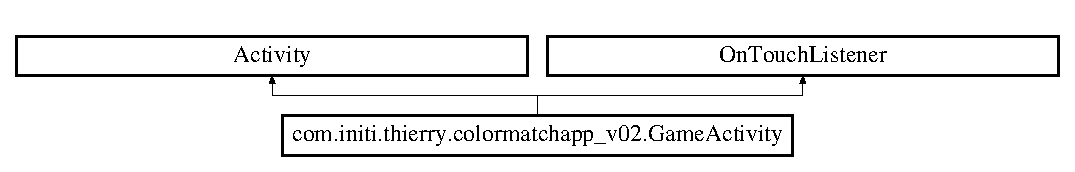
\includegraphics[height=1.866667cm]{classcom_1_1initi_1_1thierry_1_1colormatchapp__v02_1_1_game_activity}
\end{center}
\end{figure}
\subsection*{Classes}
\begin{DoxyCompactItemize}
\item 
class \hyperlink{classcom_1_1initi_1_1thierry_1_1colormatchapp__v02_1_1_game_activity_1_1_message_handler}{Message\+Handler}
\end{DoxyCompactItemize}
\subsection*{Public Member Functions}
\begin{DoxyCompactItemize}
\item 
boolean {\bfseries on\+Touch} (View v, Motion\+Event event)\hypertarget{classcom_1_1initi_1_1thierry_1_1colormatchapp__v02_1_1_game_activity_a35978f8a04e8d110025578a6c557fb92}{}\label{classcom_1_1initi_1_1thierry_1_1colormatchapp__v02_1_1_game_activity_a35978f8a04e8d110025578a6c557fb92}

\item 
void {\bfseries set\+End\+Screen} ()\hypertarget{classcom_1_1initi_1_1thierry_1_1colormatchapp__v02_1_1_game_activity_a940896f4e20418492d3458ac828d1f6b}{}\label{classcom_1_1initi_1_1thierry_1_1colormatchapp__v02_1_1_game_activity_a940896f4e20418492d3458ac828d1f6b}

\end{DoxyCompactItemize}
\subsection*{Protected Member Functions}
\begin{DoxyCompactItemize}
\item 
void {\bfseries on\+Create} (Bundle saved\+Instance\+State)\hypertarget{classcom_1_1initi_1_1thierry_1_1colormatchapp__v02_1_1_game_activity_a8e612beece821db2ee7a139252e40bad}{}\label{classcom_1_1initi_1_1thierry_1_1colormatchapp__v02_1_1_game_activity_a8e612beece821db2ee7a139252e40bad}

\item 
void {\bfseries on\+Pause} ()\hypertarget{classcom_1_1initi_1_1thierry_1_1colormatchapp__v02_1_1_game_activity_afa0bea38dc5c22ceecaf2ba56b73ee16}{}\label{classcom_1_1initi_1_1thierry_1_1colormatchapp__v02_1_1_game_activity_afa0bea38dc5c22ceecaf2ba56b73ee16}

\end{DoxyCompactItemize}


The documentation for this class was generated from the following file\+:\begin{DoxyCompactItemize}
\item 
Game\+Activity.\+java\end{DoxyCompactItemize}

\hypertarget{classcom_1_1initi_1_1thierry_1_1colormatchapp__v02_1_1_game_result_activity}{}\section{com.\+initi.\+thierry.\+colormatchapp\+\_\+v02.\+Game\+Result\+Activity Class Reference}
\label{classcom_1_1initi_1_1thierry_1_1colormatchapp__v02_1_1_game_result_activity}\index{com.\+initi.\+thierry.\+colormatchapp\+\_\+v02.\+Game\+Result\+Activity@{com.\+initi.\+thierry.\+colormatchapp\+\_\+v02.\+Game\+Result\+Activity}}
Inheritance diagram for com.\+initi.\+thierry.\+colormatchapp\+\_\+v02.\+Game\+Result\+Activity\+:\begin{figure}[H]
\begin{center}
\leavevmode
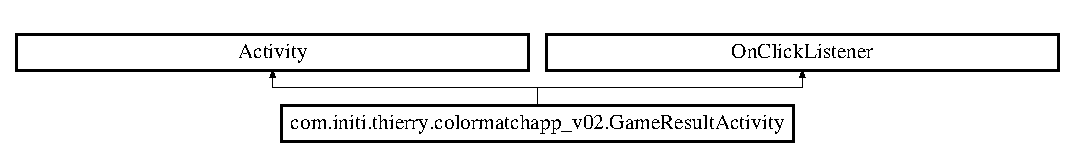
\includegraphics[height=1.676647cm]{classcom_1_1initi_1_1thierry_1_1colormatchapp__v02_1_1_game_result_activity}
\end{center}
\end{figure}
\subsection*{Public Member Functions}
\begin{DoxyCompactItemize}
\item 
void {\bfseries get\+Information} ()\hypertarget{classcom_1_1initi_1_1thierry_1_1colormatchapp__v02_1_1_game_result_activity_aeba33a68079a549118052e3a180268d7}{}\label{classcom_1_1initi_1_1thierry_1_1colormatchapp__v02_1_1_game_result_activity_aeba33a68079a549118052e3a180268d7}

\item 
void {\bfseries on\+Click} (View v)\hypertarget{classcom_1_1initi_1_1thierry_1_1colormatchapp__v02_1_1_game_result_activity_a261a53afc0ec589d6520259d7c695298}{}\label{classcom_1_1initi_1_1thierry_1_1colormatchapp__v02_1_1_game_result_activity_a261a53afc0ec589d6520259d7c695298}

\end{DoxyCompactItemize}
\subsection*{Protected Member Functions}
\begin{DoxyCompactItemize}
\item 
void {\bfseries on\+Create} (Bundle saved\+Instance\+State)\hypertarget{classcom_1_1initi_1_1thierry_1_1colormatchapp__v02_1_1_game_result_activity_ac304c5a6617a296b6e33aa183e059ea5}{}\label{classcom_1_1initi_1_1thierry_1_1colormatchapp__v02_1_1_game_result_activity_ac304c5a6617a296b6e33aa183e059ea5}

\end{DoxyCompactItemize}


The documentation for this class was generated from the following file\+:\begin{DoxyCompactItemize}
\item 
Game\+Result\+Activity.\+java\end{DoxyCompactItemize}

\hypertarget{classcom_1_1initi_1_1thierry_1_1colormatchapp__v02_1_1_game_surface}{}\section{com.\+initi.\+thierry.\+colormatchapp\+\_\+v02.\+Game\+Surface Class Reference}
\label{classcom_1_1initi_1_1thierry_1_1colormatchapp__v02_1_1_game_surface}\index{com.\+initi.\+thierry.\+colormatchapp\+\_\+v02.\+Game\+Surface@{com.\+initi.\+thierry.\+colormatchapp\+\_\+v02.\+Game\+Surface}}
Inheritance diagram for com.\+initi.\+thierry.\+colormatchapp\+\_\+v02.\+Game\+Surface\+:\begin{figure}[H]
\begin{center}
\leavevmode
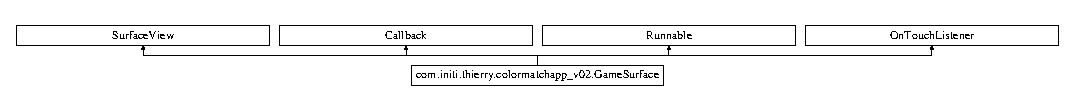
\includegraphics[height=0.924092cm]{classcom_1_1initi_1_1thierry_1_1colormatchapp__v02_1_1_game_surface}
\end{center}
\end{figure}
\subsection*{Public Member Functions}
\begin{DoxyCompactItemize}
\item 
{\bfseries Game\+Surface} (Context context)\hypertarget{classcom_1_1initi_1_1thierry_1_1colormatchapp__v02_1_1_game_surface_a5d23dec0556d5643be6ed8987fb3b5f2}{}\label{classcom_1_1initi_1_1thierry_1_1colormatchapp__v02_1_1_game_surface_a5d23dec0556d5643be6ed8987fb3b5f2}

\item 
{\bfseries Game\+Surface} (Context context, Attribute\+Set attrs)\hypertarget{classcom_1_1initi_1_1thierry_1_1colormatchapp__v02_1_1_game_surface_ab623e19555a76b8987d7f6a0708e1beb}{}\label{classcom_1_1initi_1_1thierry_1_1colormatchapp__v02_1_1_game_surface_ab623e19555a76b8987d7f6a0708e1beb}

\item 
{\bfseries Game\+Surface} (Context context, Attribute\+Set attrs, int def\+Style)\hypertarget{classcom_1_1initi_1_1thierry_1_1colormatchapp__v02_1_1_game_surface_a1019bd552ba166d34f25edbdd734773b}{}\label{classcom_1_1initi_1_1thierry_1_1colormatchapp__v02_1_1_game_surface_a1019bd552ba166d34f25edbdd734773b}

\item 
void {\bfseries init} ()\hypertarget{classcom_1_1initi_1_1thierry_1_1colormatchapp__v02_1_1_game_surface_a025b97dcdf84e6e1b6ee5d52fddcffc8}{}\label{classcom_1_1initi_1_1thierry_1_1colormatchapp__v02_1_1_game_surface_a025b97dcdf84e6e1b6ee5d52fddcffc8}

\item 
void {\bfseries load\+Board} ()\hypertarget{classcom_1_1initi_1_1thierry_1_1colormatchapp__v02_1_1_game_surface_ab142beb808dfa72ad94d6cb246ee8d64}{}\label{classcom_1_1initi_1_1thierry_1_1colormatchapp__v02_1_1_game_surface_ab142beb808dfa72ad94d6cb246ee8d64}

\item 
void {\bfseries draw\+Initial\+Board} (Canvas canvas)\hypertarget{classcom_1_1initi_1_1thierry_1_1colormatchapp__v02_1_1_game_surface_ac26644b9b3cb7e35776b3a32831a9250}{}\label{classcom_1_1initi_1_1thierry_1_1colormatchapp__v02_1_1_game_surface_ac26644b9b3cb7e35776b3a32831a9250}

\item 
void {\bfseries draw\+Squares\+On\+Board} (Canvas canvas)\hypertarget{classcom_1_1initi_1_1thierry_1_1colormatchapp__v02_1_1_game_surface_a320fceaeaad6b0c84a7cad03365e0515}{}\label{classcom_1_1initi_1_1thierry_1_1colormatchapp__v02_1_1_game_surface_a320fceaeaad6b0c84a7cad03365e0515}

\item 
boolean {\bfseries is\+Board\+Empty} ()\hypertarget{classcom_1_1initi_1_1thierry_1_1colormatchapp__v02_1_1_game_surface_a616e2611e109b6056cc4824ccf054ac3}{}\label{classcom_1_1initi_1_1thierry_1_1colormatchapp__v02_1_1_game_surface_a616e2611e109b6056cc4824ccf054ac3}

\item 
boolean {\bfseries is\+There\+Possibility} ()\hypertarget{classcom_1_1initi_1_1thierry_1_1colormatchapp__v02_1_1_game_surface_acf676d8ab2a2c34f3cc37b00abfee86a}{}\label{classcom_1_1initi_1_1thierry_1_1colormatchapp__v02_1_1_game_surface_acf676d8ab2a2c34f3cc37b00abfee86a}

\item 
void \hyperlink{classcom_1_1initi_1_1thierry_1_1colormatchapp__v02_1_1_game_surface_af3534f95e7e4bc5e9dc44920a392150e}{game\+Calculator} (int x\+Indice, int y\+Indice)
\item 
void \hyperlink{classcom_1_1initi_1_1thierry_1_1colormatchapp__v02_1_1_game_surface_a3de4bdb989882f536ea730b8a400becc}{draw\+Score} (Canvas c)
\item 
void {\bfseries draw\+Game\+Over} (Canvas canvas)\hypertarget{classcom_1_1initi_1_1thierry_1_1colormatchapp__v02_1_1_game_surface_ab32b7ae7724c4dea1c2541cf5402dc55}{}\label{classcom_1_1initi_1_1thierry_1_1colormatchapp__v02_1_1_game_surface_ab32b7ae7724c4dea1c2541cf5402dc55}

\item 
void {\bfseries draw\+Progress\+Bar} (Canvas canvas)\hypertarget{classcom_1_1initi_1_1thierry_1_1colormatchapp__v02_1_1_game_surface_acbf245e0fd7e30e373c89c89d6bb68b8}{}\label{classcom_1_1initi_1_1thierry_1_1colormatchapp__v02_1_1_game_surface_acbf245e0fd7e30e373c89c89d6bb68b8}

\item 
void {\bfseries surface\+Created} (Surface\+Holder holder)\hypertarget{classcom_1_1initi_1_1thierry_1_1colormatchapp__v02_1_1_game_surface_a76c1316607e34ad8e5ff97c621e9fdc8}{}\label{classcom_1_1initi_1_1thierry_1_1colormatchapp__v02_1_1_game_surface_a76c1316607e34ad8e5ff97c621e9fdc8}

\item 
void {\bfseries surface\+Changed} (Surface\+Holder holder, int format, int width, int height)\hypertarget{classcom_1_1initi_1_1thierry_1_1colormatchapp__v02_1_1_game_surface_ae7f2d9491b53622da295cbdc861a6c17}{}\label{classcom_1_1initi_1_1thierry_1_1colormatchapp__v02_1_1_game_surface_ae7f2d9491b53622da295cbdc861a6c17}

\item 
void {\bfseries surface\+Destroyed} (Surface\+Holder holder)\hypertarget{classcom_1_1initi_1_1thierry_1_1colormatchapp__v02_1_1_game_surface_a633b7d6234d5ce5feb78c5f0751a7cf8}{}\label{classcom_1_1initi_1_1thierry_1_1colormatchapp__v02_1_1_game_surface_a633b7d6234d5ce5feb78c5f0751a7cf8}

\item 
void {\bfseries pause} ()\hypertarget{classcom_1_1initi_1_1thierry_1_1colormatchapp__v02_1_1_game_surface_a501331bb0b325c076046a01043f660b8}{}\label{classcom_1_1initi_1_1thierry_1_1colormatchapp__v02_1_1_game_surface_a501331bb0b325c076046a01043f660b8}

\item 
boolean {\bfseries on\+Touch} (View v, Motion\+Event event)\hypertarget{classcom_1_1initi_1_1thierry_1_1colormatchapp__v02_1_1_game_surface_afce37a3716f84ddf234ef7b9dbc895a9}{}\label{classcom_1_1initi_1_1thierry_1_1colormatchapp__v02_1_1_game_surface_afce37a3716f84ddf234ef7b9dbc895a9}

\item 
void {\bfseries save\+Information} ()\hypertarget{classcom_1_1initi_1_1thierry_1_1colormatchapp__v02_1_1_game_surface_adff33b9c2ae913f01bb569c35dda14d7}{}\label{classcom_1_1initi_1_1thierry_1_1colormatchapp__v02_1_1_game_surface_adff33b9c2ae913f01bb569c35dda14d7}

\item 
void {\bfseries draw\+All} (Canvas c)\hypertarget{classcom_1_1initi_1_1thierry_1_1colormatchapp__v02_1_1_game_surface_a5b04a210d9697090c3b31ea7a25ebb10}{}\label{classcom_1_1initi_1_1thierry_1_1colormatchapp__v02_1_1_game_surface_a5b04a210d9697090c3b31ea7a25ebb10}

\item 
void {\bfseries run} ()\hypertarget{classcom_1_1initi_1_1thierry_1_1colormatchapp__v02_1_1_game_surface_a3dd15ceec75d03e7e9af5d7160d6b71a}{}\label{classcom_1_1initi_1_1thierry_1_1colormatchapp__v02_1_1_game_surface_a3dd15ceec75d03e7e9af5d7160d6b71a}

\end{DoxyCompactItemize}


\subsection{Detailed Description}
Created by Thierry on 11/25/2015. 

\subsection{Member Function Documentation}
\index{com\+::initi\+::thierry\+::colormatchapp\+\_\+v02\+::\+Game\+Surface@{com\+::initi\+::thierry\+::colormatchapp\+\_\+v02\+::\+Game\+Surface}!draw\+Score@{draw\+Score}}
\index{draw\+Score@{draw\+Score}!com\+::initi\+::thierry\+::colormatchapp\+\_\+v02\+::\+Game\+Surface@{com\+::initi\+::thierry\+::colormatchapp\+\_\+v02\+::\+Game\+Surface}}
\subsubsection[{\texorpdfstring{draw\+Score(\+Canvas c)}{drawScore(Canvas c)}}]{\setlength{\rightskip}{0pt plus 5cm}void com.\+initi.\+thierry.\+colormatchapp\+\_\+v02.\+Game\+Surface.\+draw\+Score (
\begin{DoxyParamCaption}
\item[{Canvas}]{c}
\end{DoxyParamCaption}
)\hspace{0.3cm}{\ttfamily [inline]}}\hypertarget{classcom_1_1initi_1_1thierry_1_1colormatchapp__v02_1_1_game_surface_a3de4bdb989882f536ea730b8a400becc}{}\label{classcom_1_1initi_1_1thierry_1_1colormatchapp__v02_1_1_game_surface_a3de4bdb989882f536ea730b8a400becc}
Dessine le score du joueur 
\begin{DoxyParams}{Parameters}
{\em c} & \\
\hline
\end{DoxyParams}
\index{com\+::initi\+::thierry\+::colormatchapp\+\_\+v02\+::\+Game\+Surface@{com\+::initi\+::thierry\+::colormatchapp\+\_\+v02\+::\+Game\+Surface}!game\+Calculator@{game\+Calculator}}
\index{game\+Calculator@{game\+Calculator}!com\+::initi\+::thierry\+::colormatchapp\+\_\+v02\+::\+Game\+Surface@{com\+::initi\+::thierry\+::colormatchapp\+\_\+v02\+::\+Game\+Surface}}
\subsubsection[{\texorpdfstring{game\+Calculator(int x\+Indice, int y\+Indice)}{gameCalculator(int xIndice, int yIndice)}}]{\setlength{\rightskip}{0pt plus 5cm}void com.\+initi.\+thierry.\+colormatchapp\+\_\+v02.\+Game\+Surface.\+game\+Calculator (
\begin{DoxyParamCaption}
\item[{int}]{x\+Indice, }
\item[{int}]{y\+Indice}
\end{DoxyParamCaption}
)\hspace{0.3cm}{\ttfamily [inline]}}\hypertarget{classcom_1_1initi_1_1thierry_1_1colormatchapp__v02_1_1_game_surface_af3534f95e7e4bc5e9dc44920a392150e}{}\label{classcom_1_1initi_1_1thierry_1_1colormatchapp__v02_1_1_game_surface_af3534f95e7e4bc5e9dc44920a392150e}
Met a jour le tableau et ses element selon la position y et x 
\begin{DoxyParams}{Parameters}
{\em x\+Indice} & \\
\hline
{\em y\+Indice} & \\
\hline
\end{DoxyParams}


The documentation for this class was generated from the following file\+:\begin{DoxyCompactItemize}
\item 
Game\+Surface.\+java\end{DoxyCompactItemize}

\hypertarget{classcom_1_1initi_1_1thierry_1_1colormatchapp__v02_1_1_high_score_data}{}\section{com.\+initi.\+thierry.\+colormatchapp\+\_\+v02.\+High\+Score\+Data Class Reference}
\label{classcom_1_1initi_1_1thierry_1_1colormatchapp__v02_1_1_high_score_data}\index{com.\+initi.\+thierry.\+colormatchapp\+\_\+v02.\+High\+Score\+Data@{com.\+initi.\+thierry.\+colormatchapp\+\_\+v02.\+High\+Score\+Data}}
\subsection*{Classes}
\begin{DoxyCompactItemize}
\item 
class {\bfseries Table\+Info}
\end{DoxyCompactItemize}


\subsection{Detailed Description}
Created by Thierry on 1/1/2016. 

The documentation for this class was generated from the following file\+:\begin{DoxyCompactItemize}
\item 
High\+Score\+Data.\+java\end{DoxyCompactItemize}

\hypertarget{classcom_1_1initi_1_1thierry_1_1colormatchapp__v02_1_1_main_activity}{}\section{com.\+initi.\+thierry.\+colormatchapp\+\_\+v02.\+Main\+Activity Class Reference}
\label{classcom_1_1initi_1_1thierry_1_1colormatchapp__v02_1_1_main_activity}\index{com.\+initi.\+thierry.\+colormatchapp\+\_\+v02.\+Main\+Activity@{com.\+initi.\+thierry.\+colormatchapp\+\_\+v02.\+Main\+Activity}}
Inheritance diagram for com.\+initi.\+thierry.\+colormatchapp\+\_\+v02.\+Main\+Activity\+:\begin{figure}[H]
\begin{center}
\leavevmode
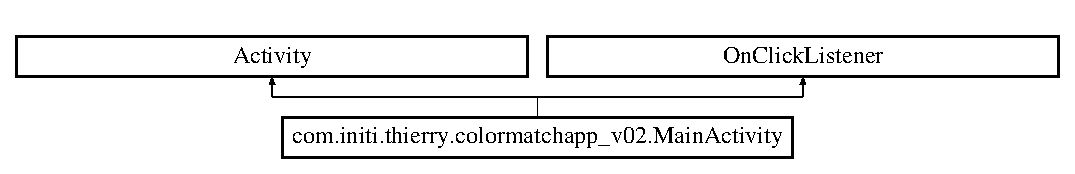
\includegraphics[height=1.891892cm]{classcom_1_1initi_1_1thierry_1_1colormatchapp__v02_1_1_main_activity}
\end{center}
\end{figure}
\subsection*{Public Member Functions}
\begin{DoxyCompactItemize}
\item 
void {\bfseries on\+Click} (View v)\hypertarget{classcom_1_1initi_1_1thierry_1_1colormatchapp__v02_1_1_main_activity_a2b16e484fd259228bbf1cc6ee42d8eab}{}\label{classcom_1_1initi_1_1thierry_1_1colormatchapp__v02_1_1_main_activity_a2b16e484fd259228bbf1cc6ee42d8eab}

\end{DoxyCompactItemize}
\subsection*{Protected Member Functions}
\begin{DoxyCompactItemize}
\item 
void {\bfseries on\+Create} (Bundle saved\+Instance\+State)\hypertarget{classcom_1_1initi_1_1thierry_1_1colormatchapp__v02_1_1_main_activity_ae0bd870462110982d9a4b3bc389b8f39}{}\label{classcom_1_1initi_1_1thierry_1_1colormatchapp__v02_1_1_main_activity_ae0bd870462110982d9a4b3bc389b8f39}

\item 
void {\bfseries on\+Pause} ()\hypertarget{classcom_1_1initi_1_1thierry_1_1colormatchapp__v02_1_1_main_activity_a184047863eec0aa27c4d41a3e5a37529}{}\label{classcom_1_1initi_1_1thierry_1_1colormatchapp__v02_1_1_main_activity_a184047863eec0aa27c4d41a3e5a37529}

\end{DoxyCompactItemize}


The documentation for this class was generated from the following file\+:\begin{DoxyCompactItemize}
\item 
Main\+Activity.\+java\end{DoxyCompactItemize}

\hypertarget{classcom_1_1initi_1_1thierry_1_1colormatchapp__v02_1_1_game_activity_1_1_message_handler}{}\section{com.\+initi.\+thierry.\+colormatchapp\+\_\+v02.\+Game\+Activity.\+Message\+Handler Class Reference}
\label{classcom_1_1initi_1_1thierry_1_1colormatchapp__v02_1_1_game_activity_1_1_message_handler}\index{com.\+initi.\+thierry.\+colormatchapp\+\_\+v02.\+Game\+Activity.\+Message\+Handler@{com.\+initi.\+thierry.\+colormatchapp\+\_\+v02.\+Game\+Activity.\+Message\+Handler}}
Inheritance diagram for com.\+initi.\+thierry.\+colormatchapp\+\_\+v02.\+Game\+Activity.\+Message\+Handler\+:\begin{figure}[H]
\begin{center}
\leavevmode
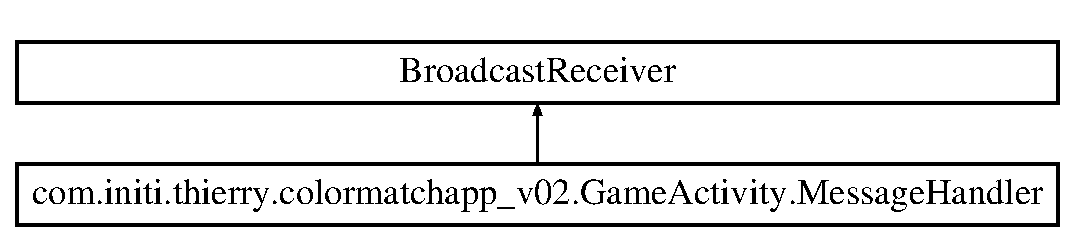
\includegraphics[height=2.000000cm]{classcom_1_1initi_1_1thierry_1_1colormatchapp__v02_1_1_game_activity_1_1_message_handler}
\end{center}
\end{figure}
\subsection*{Public Member Functions}
\begin{DoxyCompactItemize}
\item 
void {\bfseries on\+Receive} (Context context, Intent intent)\hypertarget{classcom_1_1initi_1_1thierry_1_1colormatchapp__v02_1_1_game_activity_1_1_message_handler_a60221e59c4655c77619a8b5332f89288}{}\label{classcom_1_1initi_1_1thierry_1_1colormatchapp__v02_1_1_game_activity_1_1_message_handler_a60221e59c4655c77619a8b5332f89288}

\end{DoxyCompactItemize}


The documentation for this class was generated from the following file\+:\begin{DoxyCompactItemize}
\item 
Game\+Activity.\+java\end{DoxyCompactItemize}

\hypertarget{classcom_1_1initi_1_1thierry_1_1colormatchapp__v02_1_1_point}{}\section{com.\+initi.\+thierry.\+colormatchapp\+\_\+v02.\+Point Class Reference}
\label{classcom_1_1initi_1_1thierry_1_1colormatchapp__v02_1_1_point}\index{com.\+initi.\+thierry.\+colormatchapp\+\_\+v02.\+Point@{com.\+initi.\+thierry.\+colormatchapp\+\_\+v02.\+Point}}
\subsection*{Public Member Functions}
\begin{DoxyCompactItemize}
\item 
{\bfseries Point} (int x, int y)\hypertarget{classcom_1_1initi_1_1thierry_1_1colormatchapp__v02_1_1_point_aa3031a426c726705b8bad437879c237c}{}\label{classcom_1_1initi_1_1thierry_1_1colormatchapp__v02_1_1_point_aa3031a426c726705b8bad437879c237c}

\item 
int {\bfseries getX} ()\hypertarget{classcom_1_1initi_1_1thierry_1_1colormatchapp__v02_1_1_point_aed6a1c43bf33d5c8cdc4f2132d5fb5fc}{}\label{classcom_1_1initi_1_1thierry_1_1colormatchapp__v02_1_1_point_aed6a1c43bf33d5c8cdc4f2132d5fb5fc}

\item 
void {\bfseries setX} (int x)\hypertarget{classcom_1_1initi_1_1thierry_1_1colormatchapp__v02_1_1_point_a82e48c44fcec1acd6c64b024f3c108fa}{}\label{classcom_1_1initi_1_1thierry_1_1colormatchapp__v02_1_1_point_a82e48c44fcec1acd6c64b024f3c108fa}

\item 
int {\bfseries getY} ()\hypertarget{classcom_1_1initi_1_1thierry_1_1colormatchapp__v02_1_1_point_a19db3dd14c3b2a33caf1ab82c0b6ae19}{}\label{classcom_1_1initi_1_1thierry_1_1colormatchapp__v02_1_1_point_a19db3dd14c3b2a33caf1ab82c0b6ae19}

\item 
void {\bfseries setY} (int y)\hypertarget{classcom_1_1initi_1_1thierry_1_1colormatchapp__v02_1_1_point_a2957093d5bde8cc1ff5e16d2ba9d9335}{}\label{classcom_1_1initi_1_1thierry_1_1colormatchapp__v02_1_1_point_a2957093d5bde8cc1ff5e16d2ba9d9335}

\end{DoxyCompactItemize}


The documentation for this class was generated from the following file\+:\begin{DoxyCompactItemize}
\item 
Point.\+java\end{DoxyCompactItemize}

%--- End generated contents ---

% Index
\backmatter
\newpage
\phantomsection
\clearemptydoublepage
\addcontentsline{toc}{chapter}{Index}
\printindex

\end{document}
